%% LyX 2.3.7 created this file.  For more info, see http://www.lyx.org/.
%% Do not edit unless you really know what you are doing.
\documentclass[11pt,oneside,czech]{book}
\usepackage{BP}

\begin{document}
\pagenumbering{roman}
\mytitlepage
%\includepdf[pages=-]{Zadani/zadani-BP-scan.pdf} 

\newpage{}
\addtocontents{toc}{~\hfill\textbf{Page}\par}
\addcontentsline{toc}{chapter}{Poděkování}
\podekovani
\prohlaseni

\newpage{}
\addcontentsline{toc}{chapter}{Abstrakt}
\abstrakt

\newpage{}
\addcontentsline{toc}{chapter}{Obsah}
\pagestyle{plain}
\tableofcontents{}

\newpage{}
\chapter*{Úvod}
\addcontentsline{toc}{chapter}{Úvod}
\textbf{Test citací:}
\cite{peruzzo_variational_2014}, \cite{mcclean_theory_2016}, \cite{nielsen_quantum_2010}, \cite{tilly_variational_2022}, \cite{feynman_simulating_1982}, \cite{feynman_quantum_1986}, \cite{nielsen_fermionic_2005}, \cite{tazi_folded_2024}, \cite{stechly_introduction_2024} \cite{qiskitextbook2023} \cite{gatesIMG} \newline
\textbf{Test braketů:} $\bra{\psi}$, $\ket{\phi}$, $\braket{\psi}{\phi}$, $\swch{\psi}{\hat{H}}{\phi}$, $\bra\psi \hat{H} \ket\phi$, $\swich{\psi}{\tfrac{\hat{p}^2}{2m} + \hat{V}}{\phi}$ 
\newline
\textbf{Test obvodů:} 
\newline

\begin{figure}[h]
    \centering
    \begin{quantikz}
  \lstick{\ket{0}} & \gate{H} & \ctrl{1} && \rstick[2]{$\frac{1}{\sqrt{2}}(\ket{00}+\ket{01})$} \\
  \lstick{\ket{0}} & & \targ{} &&  
\end{quantikz}
    \caption{Obvod pro vytvoření Bellových stavů.}
    \label{fig:test1}
\end{figure}

\begin{figure}[h]
    \centering
    \begin{quantikz}
   \gate[2]{Q.C.} & \slice[style = black]{} && \ctrl{1} \gategroup[2, steps = 2, style={dashed}]{\scriptsize Rotace do měřící báze} & \gate{H} & \rstick[2]{$\psi^\prime$} \\
                  &&& \targ{}  &          &  
    \end{quantikz}
    \caption{Obvod pro měření v Bellově bázi. Po aplikaci dodatečného CNOT a H odpovídá naměření $\ket{0}$ projekci původního obvodu Q.C. do stavu $\ket{+}$, obdobně naměření $\ket{1}$ odpovídá projekci do $\ket{-}$.}
    \label{fig:test2}
\end{figure}



\newpage
\pagenumbering{arabic}
\part{Teoretická část}


\chapter{Úvod do kvantové informatiky}

Rapidní vývoj klasické výpočetní techniky posledních několika dekád pravděpodobně směřuje k postupnému útlumu \mk{dost silné tvrzení. Z čeho tak soudíte? Já si to třeba nemyslím.}. (\todo{Najít nějakou seriozní referenci}) Je tedy na místě hledat alternativní technologie. Značný posun v některých typech úloh slibují kvantové počítače, které budou stručně popsány v této kapitole. Detailnější popis lze nalézt například v knize \cite{nielsen_quantum_2010}, či učebinci \cite{qiskitextbook2023}, ze kterých bylo čerpáno při zpracování této kapitoly. Před samotným popisem je však dobré si pro srovnání uvědomit pár základních faktů o počítačích klasických. Základní výpočetní jednotku a jednotku informace v nich představuje \textit{bit}, který může nabývat jednoho ze dvou stavů, obvykle označovaných $0$ a $1$. Na bity jsou aplikovány tzv. \textit{logické brány}, které mohou měnit stav bitu. Bity a brány jsou seskupovány do \textit{logických obvodů}. Teorie klasických počítačů je vybudována nezávisle na fyzické implementaci. Nezáleží, zda jsou bity a brány realizovány jako tranzistor, elektronka, či voják s vlaječkou \cite{liu2014three}. Obdobně, nezávisle na praktické realizaci, je vybudována i teorie kvantových počítačů. Základní výpočetní jednotkou a jednotkou informace je analogie bitu nazývaná \textit{kvantový bit}, jehož název je obvykle zkracován na \textit{qbit} \mk{"qubit" je mnohonásobně rozšířenější pojem. Ale je to na vás.}.   

\section{Qbit}
Qbit lze pro účely této teoretické kapitoly chápat jako matematický objekt reprezentující \mk{dvoustavový} kvantový systém. Qbit má obdobně jako klasický bit také dva možné stavy, obvykle označované $\ket{0}$ a $\ket{1}$. Na rozdíl od bitu však může nabývat i libovolné superpozice těchto stavů. 
Qbit lze chápat jako normalizovaný vektor z Hilbertova prostoru o dvou dimenzích. 

Často však pro účely kvantové informatiky používáme namísto klasické vektorové notace tzv. \textit{Diracovu (braketovou) notaci}. V této notaci \textit{ket} $\ket{\cdot}$ reprezentuje prvek nějakého Hilbertova prostoru a \textit{bra} $\bra{\cdot}$ prvek duálního prostoru k tomuto Hilbertově prostoru. Jejich spojení, \textit{braket} $\braket{\cdot}{\cdot}$ pak označuje skalární součet dvou ketů. S využitím této notace lze standardní bázi prostoru qbitu zapsat jako: 
\begin{equation}
    \bctr{1\\0} = \ket{0}, \quad \bctr{0\\1} = \ket{1}.
\end{equation}
Tato báze bývá v kvantové informatice často nazývána také \textit{standardní výpočetní báze}. Obecný stav qbitu, který je lineární kombinací těchto dvou bazických vektorů lze vyjádřit následovně:
\begin{equation}
    \ket{\psi} = \alpha \ket{0} + \beta \ket{1}, \label{eq:qbit_stav}
\end{equation}
kde $\alpha$ a $\beta$ jsou libovolná komplexní čísla, která bývají někdy nazývány \mk{spíše jsou to amplitudy z definice, než že by to byl jen název} \textit{amplitudy}. V klasické vektorové notaci má obecný stav qbitu tvar:
\begin{equation}
    \ket{\psi} = \bctr{\alpha \\ \beta}.
\end{equation}
Informaci o superpozici však nelze získat měřením\mk{špatná formulace. Čím jiným než měřením?}. Z postulátů kvantové mechaniky plyne, že měřením qbitu lze získat pouze stav $\ket 0$ s pravděpodobností $|\alpha|^2$ nebo stav $\ket 1$ s pravděpodobností $|\beta|^2$, měřením je superpozice ztracena a qbit nabude jednoho z těchto stavů. Tento mechanismus spadnutí systému do naměřeného systému bývá nazýván \textit{kolaps}. Tato statistická interpretace bývá také nazývána \textit{Bornovou interpretací} a plyne z ní omezující podmínka na koeficienty $\alpha$ a $\beta$. Musí splňovat rovnost $|\alpha|^2+|\beta|^2=1$. Stav qbitu tedy musí být normalizován.
Dalším důsledkem je irrelevance tzv. \textit{globální fáze}. Obecný stav qbitu \eqref{eq:qbit_stav} lze přepsat následujícím způsobem:
\begin{equation}
    \ket{\psi} = e^{i\gamma}\Bigl(\cos{\tfrac{\theta}{2}} \ket{0} + e^{i\varphi} \sin{\tfrac{\theta}{2}} \ket{1} \Bigr),
\end{equation}
kde jsou koeficienty $\alpha$ a $\beta$ z \eqref{eq:qbit_stav} parametrizovány úhly $\theta, \varphi$ a $\gamma$. Fáze $e^{i\varphi}$ bývá nazývána \textit{relativní fáze}, $e^{i\gamma}$ \textit{globální fáze}. Z Bornova pravidla plyne, že globální fáze nemá žádný efekt na pravděpodobnosti naměření $\ket0$, či $\ket1$. Může být proto vynechána a obecný stav v této parametrizaci je obvykle zapisován jako:
\begin{equation}
    \ket{\psi} = \cos{\tfrac{\theta}{2}} \ket{0} + e^{i\varphi} \sin{\tfrac{\theta}{2}} \ket{1}.
\end{equation}
Úhly $\varphi$ a $\theta$ charakterizují bod na \textit{Blochově sféře} vyobrazené na Obr. \ref{fig:bloch_sphere}. Jedná se o alternativní znázornění qbitu. Na této sféře póly odpovídají stavům $\ket0$ a $\ket1$. 

\begin{figure}[h]
    \centering
    \scalebox{.9}{\bloch{3}}
    \caption{Reprezentace qbitu pomocí Blochovy sféry}
    \label{fig:bloch_sphere}
\end{figure}

Dále lze na Obr. \ref{fig:bloch_sphere} pozorovat stavy $\ket+$ a $\ket-$. Tyto stavy tvoří alternativní bázi prostoru qbitu a jsou definovány jako:
\begin{equation}
    \ket{+} = \tfrac{1}{\sqrt{2}}(\ket{0}+\ket{1}), \quad \ket{-} = \tfrac{1}{\sqrt{2}}(\ket{0}-\ket{1}),
\end{equation}
případně v klasické vektorové notaci:
\begin{equation}
    \ket{+} = \tfrac{1}{\sqrt{2}}\bctr{1\\1}, \quad \ket{-} = \tfrac{1}{\sqrt{2}}\bctr{1\\-1}.
\end{equation}
Tato dvojice stavů bývá také často nazývána \textit{Hadamardova báze}. Pro popis postupu získání těchto stavů (a i jiných, obecnějších) je třeba zavést pojem \textit{kvantových bran}, které umožňují provádět operace s qbity.
\subsection{Kvantové brány}
\textit{Kvantové brány}, někdy také označovány jako \textit{Kvantová hradla} představují analogii k logickým branám na klasických počítacích. Pro jeden bit existuje pouze jedna netriviální operace, a to operace, která zneguje stav bitu (o stavech $1$ a $0$ uvažujeme jako o pravdivostních hodnotách). Tato operace je realizována logickou bránou nazývanou \textit{NOT}. 
Obdobnou operaci lze provést i na qbitu:
\begin{equation}
    \alpha \ket 0 + \beta \ket1 \rightarrow \alpha \ket 1 +\beta \ket 0,
\end{equation}
kde NOT navíc působí lineárně. Bránu, která provádí toto kvantové NOT nazýváme \textit{X brána} a lze ji reprezentovat v maticovém zápisu
\begin{equation}
    X = \begin{pmatrix*}[r] 0 & 1 \\ 1 & 0 \end{pmatrix*}.
\end{equation}
po aplikaci na obecný stav ve vektorové notaci provede operaci kvantového NOT:
\begin{equation}
    X \bctr{\alpha \\ \beta} = \bctr{\beta \\ \alpha}.
\end{equation}
Na rozdíl od klasických počítačů neexistuje pro jeden qbit pouze jedna netriviální operace. Díky vlastnosti superpozice jich dokonce existuje nekonečně mnoho \mk{jsou teorémy, že ve skutečnosti jich stačí jen pár zbytek se z nich odvodí.}. Jak bylo nastíněno v případě brány X, kvantové brány pro jeden qbit jsou reprezentovány pomocí $2$x$2$ matic. Na tyto matice je však nutno vznést určitá omezení. 

Operace na qbitech by měly ideálně být reverzibilní \mk{ne, že by "měly", ale ony jsou z toho důvodu, že musí být unitární.}. Dále by také měly \mk{opět, musí} zachovávat normalizaci stavu, aby platilo Bornovo pravidlo. Z těchto požadavků plyne, že kvantové brány musí v maticové reprezentaci odpovídat unitárním maticím. Unitární matice zachovávají normu a vždy pro ně existuje inverzní matice, která je rovna Hermitovsky sdružené matici. \mk{Tento odstavec je matoucí, obvykle řekneme, že je to unitární a z co z toho plyne. Jinak z čeho plyne, že by to mělo být reverzibilní? Zvláště pokud klasické nejsou?} Tedy pro Unitární matici platí:
\begin{equation}
    U^\dag U = I, \quad \| U\ket{\psi} \| = \swch{\psi}{U^\dag U}{\psi}^{\sfrac{1}{2}} = \sqrt{\braket{\psi}{\psi}} = 1.
\end{equation}
\mk{DOporucuji u vsech operatoru psat "hat", jak v textu tak ve vzorcich.}
Brány však nemusí být Hermitovské, a tudíž můžou, ale nemusí být zároveň i kvantovými pozorovatelnými. Další důležitou bránou je \textit{Hadamardova brána} H. Ta transformuje vektory standardní výpočetní báze na stavy $\ket +$ a $\ket -$. 
\begin{equation}
    \hat{H} \Bigl(\alpha \ket{0} + \beta \ket 1\Bigr) = \alpha \tfrac{\ket 0 + \ket 1}{\sqrt{2}}  + \beta \tfrac{\ket 0 - \ket 1}{\sqrt{2}} = \alpha \ket+ + \beta \ket-
\end{equation}
\mk{Torchu nestandardní. Osobně bych na dva řádky dal jednu aplikace na 0 a druhou na 1.}
Operaci H lze také interpretovat v reprezentaci Blochovy sféry jako rotaci o úhel $\tfrac{\pi}{2}$ kolem osy $y$ následovanou rotací o úhel $\pi$ kolem osy $x$, viz Obr. \ref{fig:bloch_sphere}. Maticové vyjádření Hadamardovy brány má tvar:
\begin{equation}
   \mk{H=} \frac{1}{\sqrt{2}} \begin{pmatrix*}[r] 1 & 1 \\ 1 & -1 \end{pmatrix*}.
\end{equation}
V notaci pro \textit{kvantové obvody}, které slouží k spojení více bran a qbitů pro složitější operace znázorňujeme Hadamardovu bránu následovně.

\begin{figure}[h]
    \centering
    \begin{quantikz}
  & \gate{H} & 
\end{quantikz}
    \caption{Notace hadamardovy brány v kvantových obvodech.}
    \label{fig:hadamard}
\end{figure}

\subsection{Pauliho Brány}
Dalšími důležitými kvantovými branami jsou Pauliho brány $X$, $Y$ a $Z$. Obdobně jako matice Hadamardovy brány jsou matice Pauliho bran, nazývané \textit{Pauliho matice}, Hermitovské a jsou tedy také kvantovými pozorovatelnými. Pojmy Pauliho brána, matice a operátor proto bývají často zaměňovány. Fyzikálně představují ve spinorové reprezentaci projekci spinu do příslušných os. Jsou-li interpretovány jako pozorovatelné, značí se obvykle $\hat{\sigma}_x$, $\hat{\sigma}_y$ a $\hat{\sigma}_z$.  Jejich matice mají tvar:
\begin{equation}
    \hat{\sigma}_x = X = \begin{pmatrix*}[r] 0 & 1 \\ 1 & 0 \end{pmatrix*}, \quad
    \hat{\sigma}_y = Y = \begin{pmatrix*}[r] 0 & i \\ -i & 0 \end{pmatrix*}, \quad
    \hat{\sigma}_z = Z = \begin{pmatrix*}[r] 1 & 0 \\ 0 & -1 \end{pmatrix*}.
\end{equation}
Notace pro kvantové obvody je zobrazena na Obr. $\ref{fig:pauli}$. Další důležitou vlastností Pauliho matic je,  že společně s identitou tvoří bázi všech $2$x$2$ matic a tudíž jejich lineární kombinací lze vytvořit libovolnou jinou kvantovou bránu. Hadamardovu bránu lze například rozepsat jako:
\begin{equation}
H = \tfrac{1}{\sqrt{2}} (X + Z). 
\end{equation}
Důležitou roli, obzvlášť pro měření kvantových pozorovatelných \textsuperscript{[\ref{sec:mereni_operatoru}]}, mají vlastní vektory a vlastní hodnoty Pauliho matic. Jejich shrnutí lze nalézt v tabulce \ref{table:eigenpauli}. Za povšimnutí stojí fakt, že vlastní vektory $Z$ odpovídají standardní výpočetní bázi. Tato báze se z tohoto důvodu někdy nazývá také \textit{Z báze}.

\begin{table}
\centering
\begin{tabular}{c|c|c|c} 
 Vl. číslo & $X$ & $Y$ & $Z$ \\
 \hline
 \hline
  & & & \\
 $\lambda = +1$ & $\tfrac{1}{\sqrt{2}}$\bctr{1 \\ 1}, $\ket+$ & $\tfrac{1}{\sqrt{2}}$\bctr{1 \\ i} & \bctr{1 \\ 0}, $\ket 0$ \\
 & & & \\
$\lambda = -1$ & $\tfrac{1}{\sqrt{2}}$\bctr{1 \\ -1}, $\ket-$ & $\tfrac{1}{\sqrt{2}}$\bctr{1 \\ -i} & \bctr{0 \\ 1}, $\ket 1$ \\
\end{tabular}
\caption{Tabulka popisující spektrum Pauliho operátorů. \mk{misto "," bych dal =}}
\label{table:eigenpauli}
\end{table}

\begin{figure}
    \centering
    \begin{quantikz} & \gate{X} & \end{quantikz}
    \begin{quantikz} & \gate{Y} & \end{quantikz}
    \begin{quantikz} & \gate{Z} & \end{quantikz}
    \caption{Notace Pauliho bran v kvantoých obvodech.}
    \label{fig:pauli}
\end{figure}

Další vlastností, důležitou obzvláště pro variační kvantové algoritmy, kterými se tato práce zabývá \textsuperscript{[\ref{sec:pauli_grouping}]} je, že po přenásobení imaginární jednotkou tvoří Pauliho matice bázi Lieovy algebry $SU(2)$ a splňují následující komutační relace
\begin{equation}
    [\hat{\sigma}_j, \hat{\sigma}_k] = 2i\varepsilon_{jkl}\hat{\sigma}_l
\end{equation}
a následující antikomutační relace
\begin{equation}
    \{ \hat{\sigma}_j, \hat{\sigma}_k \} = 2 \delta_{jk} \hat{I}.
\end{equation}

\todo{\textbf{-Rozklad brány do rotací a univerzální brány - DOPSAT!!!}} \\
\todo{\textbf{Solovay-Kitaev Theorem....asi jenom důsledky a odkaz na článek}} \\

Další kvantové brány pro jeden qbit lze nalézt na Obr. \ref{fig:gates}. Logickým krokem dopředu jsou nyní brány pro více qbitů. Před jejich zavedením je však nejprve vhodné zavést notaci pro více qbitů.



\todo{\textit{
-používáme Diracovu (Bra(c)-ketovou) notaci. \\
- Ket odpovídá vektoru z Hilbertova prostoru \\
- Bra je prvek duálního prostoru \\
- Braket představuje skalární součin. 
-Superpozice!! -> Hilbertův prostor -> paprsek, Bornovo pravidlo, pravděposobnost, normalizace \\
-výpočetní báze \\
-jiná báze - + a -, znázornit i vektorově \\
-vytvoříme pomocí hadamardovy brány \\
-brány jsou reverzibilní \\
-brány unitární \\
-pauli + hadamard zároveň i pozorovatelné \\
- X,Y,Z používáno pro brány, $\sigma_x,\  \sigma_y, \ \sigma_z$ spíše pro pozorovatelné \\
-pauli generátor SU(2) (násobené i) \\
-pauliho matice + jejich vl. stavy a čísla (obě notace) \\
-změříme qbit - kolabs do některého ze stavů \\}}

\section{Více Qbitů}
Stav dvou qbitů, z nichž jeden je ve stavu $\ket \phi$ a druhý $\ket \psi$ lze vyjádřit tenzorovým součinem těchto stavů. 
\begin{equation}
    \ket{\phi} \otimes \ket{\psi} = \ket{\phi \, \psi}, \label{eq:tensor_ket}
\end{equation}
Tento zápis bývá často zkracován do jednoho ketu \eqref{eq:tensor_ket}. Bazické vektory prostoru dvou qbitů lze získat tenzorovým součinem bazických vektorů pro prostor jednoho qbitu. Pro společný stav dvou qbitů v obecném stavu \eqref{eq:qbit_stav} po užití pravidel pro tenzoroý součin a zkrácení pomocí \eqref{eq:tensor_ket} platí:
\begin{equation}
    (\alpha_1 \ket{0} + \beta_1 \ket{1})\otimes(\alpha_2 \ket{0} + \beta_2 \ket{1}) = \alpha_1\alpha_2 \ket{00} + \alpha_1\beta_1 \ket{01} + \beta_1\alpha_2 \ket{10} + \beta_1\beta_2 \ket{11}
\end{equation}
Důležitým pozorováním je, že amplitudy tohoto stavu nejsou nezávislé. Vektory jejichž lineární kombinací je tento stav vyjádřen \eqref{eq:2qbit_baze} \mk{většinou se nedokazujeme na rovnici, která bude teprve následovat. Dal bych tu rovnici nekam výše, nebo sem.} tvoří bázi čtyřdimenzionálního Hilbertova prostoru dvou qbitů. Tato báze je rozšířením standardní báze na dva qbity a lze ji získat tenzorovým součinem jednotlivých prvků standardní báze. Identickým způsobem lze dále generovat báze pro více qbitů.
\begin{equation}
    \ket{00},\ \ket{01},\ \ket{10},\ \ket{11} \label{eq:2qbit_baze}
\end{equation}
Obdobně lze tenzorovým součinem dvou jedno-qbitových stavů ve vektorové notaci dospět k vektorové notaci pro společný stav dvou qbitů.
\begin{equation}
    \bctr{\alpha_1 \\ \beta_1} \otimes \bctr{\alpha_2 \\ \beta_2} = \bctr{\alpha_1 \alpha_2 \\ \alpha_1 \beta_2 \\ \beta_1 \alpha_2 \\ \beta_1 \beta_2}
\end{equation}
\begin{equation}
    \alpha \ket{00} + \beta \ket{01} + \gamma \ket{10} + \delta \ket{11} = \bctr{\alpha \\ \beta \\ \gamma \\ \delta}
\end{equation}
Zde se ukazuje výhoda braketové notace. Pro systém $n$ qbitů by vektor byl $2^n$ dimenzionální, což pro velká $n$ \mk{csechna $n$ kurzivou} značně znepříjemňuje zápis. Také začíná vyplývat na povrch jedna z výhod kavantových počítačů, k popisu $n$ qbitů je na klasickém počítači třeba $2^n$ amplitud. Pro $200$ qbitů je potřebný počet amplitud větší, než předpokládaný počet atomů ve vesmíru. \\ \todo{Najít v literatuře počet atomů ve vesmíru... $\approx 10^{82} - 10^{84}$}

Pro operátory působící na jeden qbit platí následující
\begin{equation}
    \hat{A} \ket{\phi} \otimes \hat{B} \ket{\psi} = (\hat{A} \otimes \hat{B}) (\ket{\phi} \otimes \ket{\psi}),
\end{equation}
tento zápis bývá často zkracován na
\begin{equation}
    \hat{A}\hat{B}\ket{\phi \psi}.
\end{equation}
\mk{u takoveho zapisu jeden musi byt opatrny, na co to pusobi. SPese se setkavam s necim jako je
\begin{equation}
    (\hat{A}\otimes\hat{B})\ket{\phi \psi}.
\end{equation}
}
Některé brány pro více qbitů tedy lze získat tenzorovým součinem bran pro jeden qbit. Brána pro $n$ qbitů bude v maticové reprezentaci odpovídat matici o rozměrech $2^n$x $2^n$.

Důležitým poznatkem pro tuto práci je, jak vypadá spektrum tenzorového součinu operátorů. Nechť $\ket{a}$, $a$ a $\ket{b}$, $b$ jsou popořadě vlastní vektor a k němu příslušné vlastní číslo operátorů $\hat{A}$ a $\hat{B}$, pak
\begin{equation}
    \hat{A} \ket{a} \otimes \hat{B} \ket{b} = a \ket{a} \otimes b \ket{b} = ab \ket{ab} = \hat{A} \hat{B} \ket{ab}.
\end{equation}
Vlastní vektory tedy odpovídají tenzorovému součinu vlastních vektorů původních operátorů a vlastní čísla odpovídají součinu příslušných vlastních čísel.

\section{Brány pro více qbitů}
\mk{Pokud se nemylim, tak vlastne staci jen CNOT a v kombinaci s jedno-qubitovymi branami pak muzete zkontruovat libovolnou 2q branu.}
Existují ale i více qbitové brány, které nelze vyjádřit jako tenzorový součin bran pro jeden qbit. Velkou skupinu takových bran tvoří \textit{kontrolované brány}. V kontrolované bráně pro dva qbity slouží první jako kontrolní qbit, v závislosti na jeho stavu je pak aplikována na druhý qbit nějaká brána. Příkladem takové brány je například \textit{CNOT} (z anglického Controlled NOT). Jedná se o kontrolovanou $\hat{X}$ bránu, pokud je stav prvního qbitu $\ket{1}$, aplikuje na druhý qbit bránu $\hat{X}$. Pokud je stav prvního qbitu $\ket{0}$, zůstává stav nezměněn. Jedná se o analogii k bráně XOR (exclusive OR) na klasických počítačích, která však obdobně jako kvantové NOT působí lineárně. Matice brány CNOT má tvar \eqref{eq:CNOT} a notace pro kvantové obvody je znázorněna na Obr. \ref{fig:CNOT}.

\begin{equation}
    CNOT = \begin{pmatrix*}[r] 1&0&0&0 \\ 0&1&0&0 \\ 0&0&0&1 \\ 0&0&1&0 \end{pmatrix*} \label{eq:CNOT}
\end{equation}

\begin{figure}[h] 
    \centering
    \begin{quantikz}
     & \ctrl{1} & \\ & \targ{}  & 
    \end{quantikz}
    \caption{Notace CNOT brány v kvantových obvodech.}
    \label{fig:CNOT}
\end{figure}
\mk{možná sem hodit obecný příklad na použití CNOT.}
Kontrolované brány mohou působit i na více qbitů. Obvykle pak aplikují nějakou jedno-qbitovou bránu na poslední qbit, a to právě tehdy pokud všechny předchozí qbity jsou ve stavu $\ket{1}$. Příkladem takové brány je \textit{Toffoliho brána}, někdy také nazývána CCNOT, která operuje na třech qbitech jako kontrolované CNOT. Je zobrazena na \ref{fig:gates} společně s dalšími často využívanými branami.


\subsection{Kvantové provázání}
Existují i stavy, které nelze rozložit pomocí tenzorového součinu. Takové stavy se nazývají \textit{provázané}. Provázání lze popsat jako určitou korelaci mezi výsledky měření jednotlivých qbitů, kdy měření jednoho qbitu ovlivní stav druhého a měření tak nelze provést nezávisle. Příkladem takových stavů jsou například Bellovy stavy. Na těchto stavech budou stručně popsány důsledky a význam provázání.
\subsection{Bellovy stavy}
\todo{\textit{
-Krátce EPR, historie \\
-Bellova báze \\
-Stručně Quantum teleportation \\}}

\begin{align}
    \ket{\psi_{00}} & = \tfrac{1}{\sqrt{2}} (\ket{00} + \ket{11}) \\
    \ket{\psi_{01}} & = \tfrac{1}{\sqrt{2}} (\ket{01} + \ket{10}) \\
    \ket{\psi_{10}} & = \tfrac{1}{\sqrt{2}} (\ket{00} - \ket{11}) \\
    \ket{\psi_{11}} & = \tfrac{1}{\sqrt{2}} (\ket{01} - \ket{10}) 
\end{align}


\begin{figure}[h]
    \centering
    \begin{quantikz}
  \lstick{\ket{0}} & \gate{H} & \ctrl{1} && \rstick[2]{$\frac{1}{\sqrt{2}}(\ket{00}+\ket{11})$} \\
  \lstick{\ket{0}} & & \targ{} &&  
\end{quantikz}
    \caption{Obvod pro vytvoření Bellových stavů.}
    \label{fig:bell_states}
\end{figure}

\subsection{No-clonning theorem}
\section{Kvantový paralelismus}
\todo{\textit{- vyvrátit popular misconception - kvanotvé počítače počítají paralelně všechny možnosti \\
-mohou pracovat se superponovanými stavy, k nim ale nemáme přístup \\
-nakonec musíme stejně provést projekční měření a systém nám zkolabuje \\
-výhodu oproti klasickým získáme tak, že se systémem chytře pracujeme a získáme část skryté informace o superpozici \\
-popsat Deutsche....možná?
}}
\section{Kvantové obvody}
Jak již bylo naznačeno, k provádění složitějších operací na qbitech složením více kvantových bran slouží \textit{kvantové obvody}. \mk{Ja bych to ppsal z opačného konce, tedy že soustava kvantových bran tvoří obvod.} Na rozdíl od klasických logických obvodů jsou kvantové obvody lineární v tom smyslu, že nepovolují žádné smyčky.\mk{To už také není úplně pravda, jsou tu triky za použití tzv. mid-circuit measurement.} Jejich dalšími důležitými vlastnostmi jsou reverzibilita a unitarita, které plynou z faktu, že kvantové obvody jsou pouze sérií unitárních kvantových bran aplikovaných na set qbitů. Z tohoto faktu také plyne možnost vyjádřit kvantový obvod unitární maticí.

Kvantový obvod se sestává z několika částí. Na vstupu obvodu se nachází \textit{kvantový registr}, soubor qbitů na kterých obvod operuje. Poté je zde samotné tělo obvodu které obsahuje jednotlivé kvantové brány. Obvod obsahuje také \textit{klasický registr}, který slouží pro odečítání hodnot z měření. 

Obvody zakreslujeme pomocí diagramů, viz např. Obr. \ref{fig:bell_states}. Obvody čteme zleva a jednotlivé horizontální čáry reprezentují qbity. Do obvodu také zakreslujeme měření, a to pomocí následujícího symbolu.

\mk{Když takto pěkně popisuje obvody, tak napište i co znamená šířka a hloubka kvantového obvodu.}

\begin{figure}[h] 
    \centering
    \begin{quantikz}
     & \meter{} & 
    \end{quantikz}
\end{figure}

\begin{figure}
    \centering
    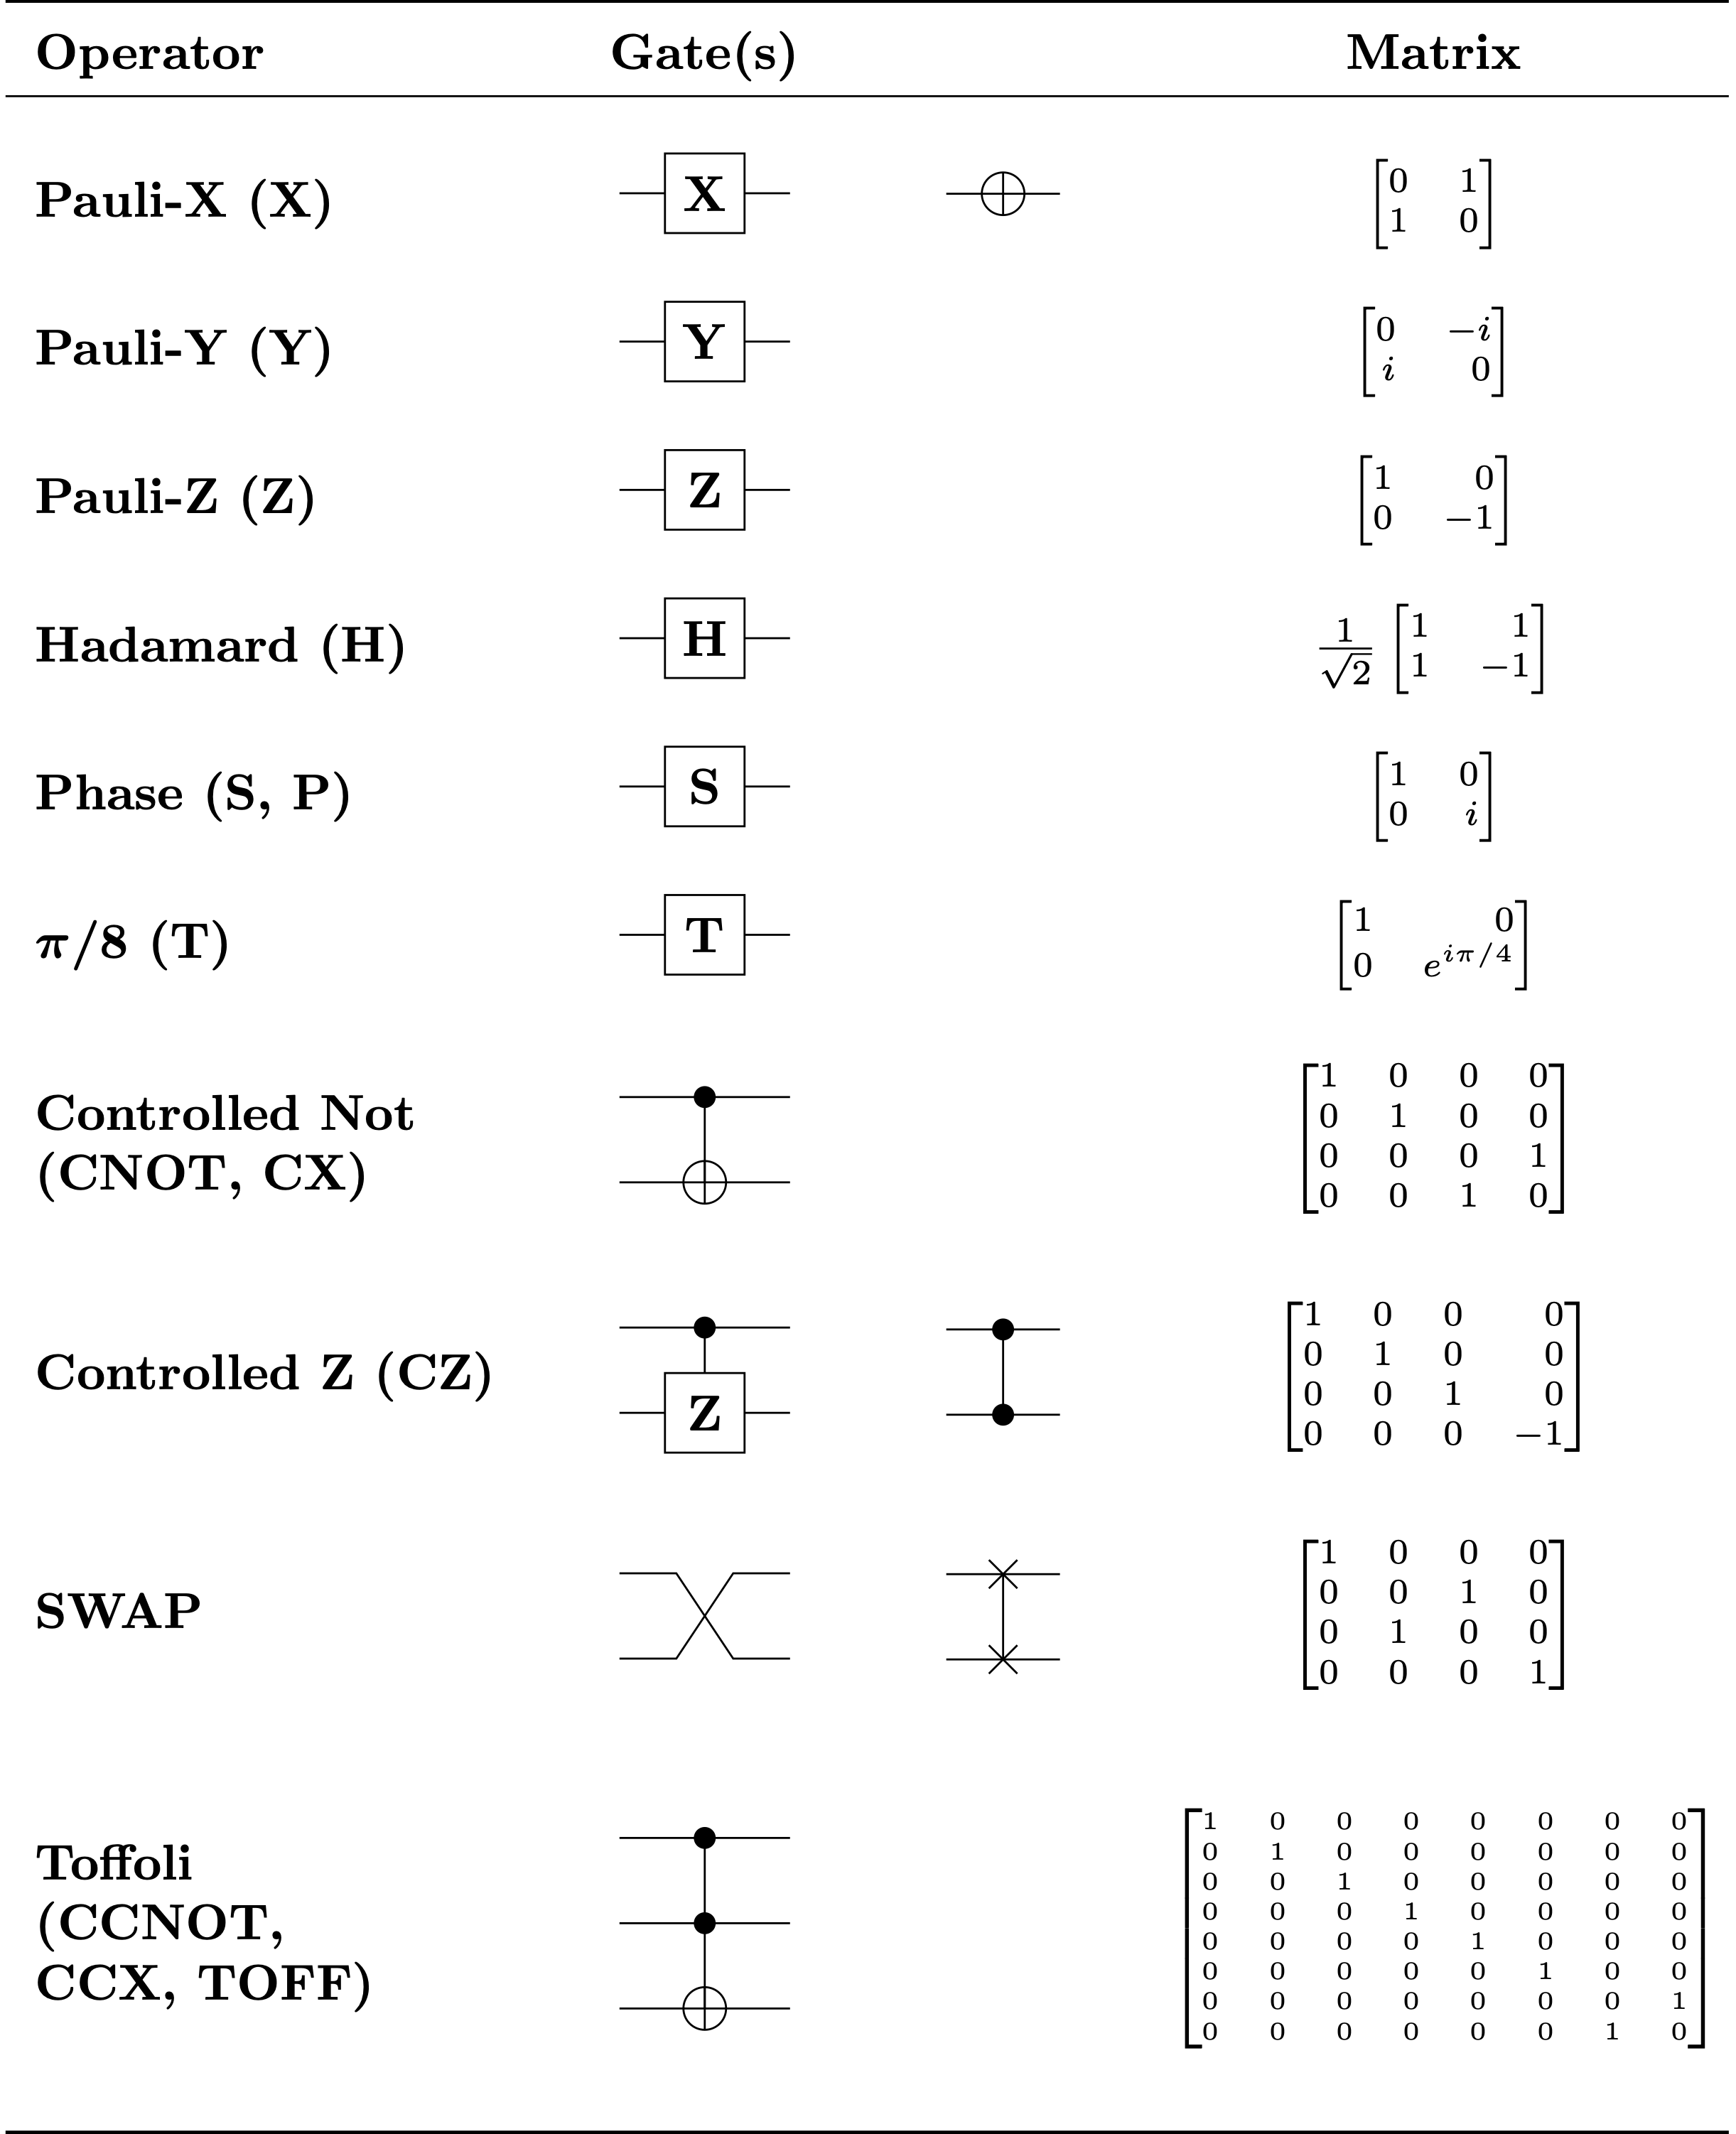
\includegraphics[width = 0.7\textwidth]{Images/Quantum_Logic_Gates.png} 
    \caption{ukradeno z \cite{gatesIMG}}
    \label{fig:gates}
\end{figure}

\mk{u obrazku doporucuji vzdy nastavit [htb] za {figure}}

\section{Měření na kvantovém počítači} \label{sec:measurement}
\todo{V závislosti na definici pojmu informace lze stav qbitu interpretovat i tak, že jeho pomocí lze kódovat nekonečně množství informace. To však nelze z qbitu žádným způsobem extrahovat, jelikož měřením lze získat pouze některý ze stavů výpočetní báze. Měřením systém navíc zkolabuje do naměřeného stavu.}


Měření na kvantovém počítači je vždy ve vztahu k nějaké bázi. Na kvantových počítačích je většinou pro měření užívána standardní báze. Měření qbitu ve standardní bázi matematicky odpovídá aplikaci projekčních operátorů:
\begin{equation}
    \hat{P}_0 = \p{0}, \quad \hat{P}_1 = \p{1}.
\end{equation}
Tyto operace nejsou unitární, nelze je tak interpretovat jako kvantovou bránu. Po měření systém (obvod) \mk{obvod určitě ne. BUď kvantový stav nebo qubit} zkolabuje do naměřeného stavu. 

Stav obvodu \mk{obvod určitě ne, ale kvantový stav.} lze částečně zrekonstruovat pomocí opakovaného měření. Kvůli kolapsu stavu po měření musí být však před každým opakování qbity v obvodu připraveny do měřeného stavu znovu. Tímto opakovaným měřením je vygenerována distribuce naměřených výsledků. Normalizací této distribuce  přibližné pravděpodobnosti naměření jednotlivých prvků standardní báze. Z nich pak lze umocněním získat amplitudy náležící k jednotlivým bazickým stavům.


\begin{figure}[H]
\begin{subfigure}{0.4\textwidth}
        \centering
        \begin{quantikz}
  \lstick{\ket{0}} & \gate{H} & \ctrl{1} &\meter{} &  \\
  \lstick{\ket{0}} & & \targ{} & \meter{} &  
\end{quantikz}
\vspace{2cm}
    \caption{Second subfigure.}
    \label{fig:second}
\end{subfigure}
\begin{subfigure}{0.4\textwidth}
    \centering
    \begin{tikzpicture}
\begin{axis}[
    symbolic x coords={$\ket{00}$, $\ket{01}$, $\ket{10}$, $\ket{11}$},
        ylabel = {Počet měření},
        xlabel = {Stav},
        xtick=data]
    \addplot[ybar,fill=white] coordinates {
        ($\ket{00}$,499)
        ($\ket{01}$,0)
        ($\ket{10}$,0)
        ($\ket{11}$,501)
    };
\end{axis}
\end{tikzpicture}
    \caption{Third subfigure.}
    \label{fig:third}
\end{subfigure}
\caption{Placeholder...udělat graf v matplotlib}
\label{fig:measurement_explanation}
\end{figure}

\todo{Ilustrační příklad toho, že projekci do jiné báze z měření ve standardní bázi prostě nedostanem:}

Na kvantovém počítači tvořeném jedním qbitem, který nám připravuje systém do neznámého stavu $\ket{\psi}$ bylo provedeno $100000$ měření s následujícími výsledky:
\begin{equation*}
    \ket{0}: 36000 \quad \ket{1}: 64000.
\end{equation*}
Tedy stav $\ket{0}$ s pravděpodobností přibližně $\tfrac{9}{25}$ a $\ket{1}$ s pravděpodobností $\tfrac{16}{25}$. Nyní bychom rádi učinili odhad velikosti projekce $\braket{+}{\psi}$ s využitím tohoto měření. Stav $\ket{\psi}$ můžeme aproximovat jako:
\begin{equation}
    \ket{\psi} \approx \tfrac{3}{5} \ket{0} + e^{i\theta} \tfrac{4}{5} \ket{1}
\end{equation}
Fáze $e^{i\theta}$ nijak neovlivní pravděpodobnosti naměření $\ket{0}$ či $\ket{1}$, její norma je totiž rovna $1$. Nyní použijeme transformační vztahy mezi standardní a Hadamardovou bazí:
\begin{equation}
    \ket{0} = \frac{\ket{+} + \ket{-}}{\sqrt{2}}, \quad
    \ket{1} = \frac{\ket{+} - \ket{-}}{\sqrt{2}}
\end{equation}
Získáme tak stav $\ket{\psi}$ ve tvaru:
\begin{equation}
    \ket{\psi} = \frac{3+4e^{i\theta}}{5\sqrt{2}} \ket{+} + \frac{3-4e^{i\theta}}{5\sqrt{2}} \ket{-}
\end{equation}
Zde ale již Fourierovy koeficienty závisí na fázi $e^{i\theta}$. Pravděpodobnost naměření stavu $\ket{+}$ se tak v závislosti na parametru $\theta$ může pohybovat mezi $\tfrac{2}{100}$ pro $\theta = \pi$ a $\tfrac{98}{100}$ pro $\theta = 0$. Tímto měřením jsme tedy nezískali žádnou informaci o zastoupení $\ket{+}$ a $\ket{-}$ ve stavu $\psi$.

Tento postup je tedy pro měření v jiné než standardní bázi nevhodný. Pro měření v jiné bázi musíme provést dodatečné operace. 

\subsection{Měření v Bázi}
\todo{-Poro měření v bázi musíme výsledný stav obvodu zrotovat tak, aby báze ve které chceme měřit odpovídala standardní. \\
-Lze využít invertibility obvodu a přilepit inverzi obvodu pro vytvoření báze ve které chceme měřit}

Hadamardova matice je unitární a symetrická. Její inverze je tedy rovna 

\begin{figure}[h]
    \centering
    \begin{quantikz}
   \gate[2]{Q.C.} & \slice[style = black]{} && \gate{H} \gategroup[1, steps = 1, style={dashed}]{\scriptsize Rotace do měřící báze} & \rstick[2]{$\psi^\prime$}
    \end{quantikz}
    \caption{Obvod pro měření v Hadamardově bázi. Po aplikaci dodatečného CNOT a H odpovídá naměření $\ket{0}$ projekci původního obvodu Q.C. do stavu $\ket{+}$, obdobně naměření $\ket{1}$ odpovídá projekci do $\ket{-}$.}
    \label{fig:hadamard_measurement}
\end{figure}

Často také říkáme, že pro měření provedeme rotaci do Z báze. Z báze představuje standartní bázi (vl. vektory $\sigma_z$).

\begin{figure}[h]
    \centering
    \begin{quantikz}
   \gate[2]{Q.C.} & \slice[style = black]{} && \ctrl{1} \gategroup[2, steps = 2, style={dashed}]{\scriptsize Rotace do měřící báze} & \gate{H} & \rstick[2]{$\psi^\prime$} \\
                  &&& \targ{}  &          &  
    \end{quantikz}
    \caption{Obvod pro měření v Bellově bázi.}
    \label{fig:bell_measurement}
\end{figure}


\todo{-Možnost extrahovat informace ze superpozice \\
-Příklad s fází \\
-Vysvětlení pomocí diagonalizace \\
-Vysvětlení pomocí transformace stavů (inverzní obvod k tomu co vytvoří vlastní stavy) \\}
\subsection{Měření operátorů}
\label{sec:mereni_operatoru}
Měřením operátoru rozumíme získání jeho střední (očekávané) hodnoty. Střední hodnota nás zajímá vždy v nějakém stavu. Jelikož se jedná o veličinu statistického charakteru, probíhá měření iterativně. Na kvantovém počítači připravíme stav, ve kterém nás zajímá střední hodnota operátoru a opakovaně tento stav měříme. Pomocí výsledků těchto měření jsme schopni aproximovat očekávanou hodnotu pozorovatelné.

Poznatky této části jsou pouhou aplikací teorie diagonalizace a spektrálního rozvoje. Důkazy k tvrzením lze nalézt ve většině literatury zabývající se lineární algebrou. (\todo{reference na nějakou knihu...možná modrá smrt?})

Pozorovatelné odpovídají Hermitovským operátorům. Jsou tedy diagonalizovatelné a jejich vlastní vektory tvoří kompletní ortogonální bázi. Měření v bázi, ve které je hermitovský operátor (pozorovatelná) diagonální (vlastní/přirozená báze) odpovídá měření ve standardní bázi. Abychom tedy mohli provádět měření (ve std. bázi) musíme pozorovatelné diagonalizovat. To lze provést transformací stavu před měřením. Ilustrujme měření pozorovatelné na kvantovém počítači na následujícím příkladu měření $\hat{\sigma}_x$. 

Pauliho brána $X$ je jak unitární, tak hermitovská. Představuje tedy také pozorovatelnou, například v nerelativistické kvantové mechanice ve spinorové reprezentaci pro spin $\sfrac{1}{2}$ projekci spinu do osy $x$. Tuto pozorovatelnou označujeme $\hat{\sigma}_x$. 

Mějme stav $\psi$, který jsme schopni realizovat na kvantovém počítači. Chceme změřit střední hodnotu $\hat{\sigma}_x$ v tomto stavu. Střední hodnotu pozorovatelné lze matematicky vyjádřit pomocí "diracova sandwiche":  %(\todo{možná diracův toast?})

\begin{equation}
    \swich{\psi}{\hat \sigma_x}{\psi} = \bra{\psi} \Bigl( \lambda_+ \p{+} + \lambda_- \p{-} \Bigr) \ket{\psi} = \bra{\psi} \Bigl( \p{+} - \p{-} \Bigr) \ket{\psi} = \braket{+}{\psi}^2 - \braket{-}{\psi}^2.
\end{equation}

Zde v první rovnosti provedeme spektrální rozvoj $\sigma_x$. V poslední rovnosti užijeme hermitovskosti skalárního součinu nad $\mathbb{C}$.

Problém určení střední hodnoty pozorovatelné jsme tedy převedli na určení velikostí projekcí stavu $\psi$ do stavů $\ket{+}$ a $\ket{-}$. Tento problém však byl vyřešen v předchozí podkapitole. Stačí stav $\psi$ zrotovat do správné báze aplikací dodatečné Hadamardovy brány.

\begin{equation}
    \braket{+}{\psi}^2 - \braket{-}{\psi}^2 = \swich{0}{H^\dag}{\psi}^2 - \swich{1}{H^\dag}{\psi}^2 = \braket{1}{\psi^\prime}^2 - \braket{0}{\psi^\prime}^2
\end{equation} 

V tomto případě lze transformaci i "vykoukat" ze znalosti matice přechodu mezi bazí $\ket{0}$,$\ \ket{1}$ a $\ket{+}$,$\ \ket{-}$. 





\begin{align}
    \swich{\psi}{\hat A}{\psi} &= \swich{\psi}{\hat R ^\dag \hat D \hat R}{\psi} \\
    &= \bra{\psi} \hat{R}^\dag \biggl( \sum_{j=0}^{n-1}  \swich{j}{\hat{D}}{j} \p{j} \biggr) \hat{R} \ket{\psi} \\
    &= \sum_{j=0}^{n-1} D_{jj} \swich{j}{\hat{R}}{\psi}^2 = \sum_{j=0}^{n-1} D_{jj} \braket{j}{\psi^\prime}^2
\end{align}

Operátor lze tedy diagonalizovat také přechodem do vlastní báze operátoru. V takovém případě je diagonální matice $D$ tvořena vlastními čísly a sloupce $R^\dag$ odpovídají normalizovaným vlastním vektorům. To při znalosti vlastních hodnot operátoru značně ulehčí výpočet jeho střední hodnoty.

Měření střední hodnoty operátoru $\hat{A}$ ve stavu $\psi$ na kvantovém počítači tedy probíhá následujícím způsobem. K obvodu, který připravuje stav $\psi$ přidáme brány odpovídající $\hat{R}$. Počítač tak bude simulovat stav $\ket{\psi^\prime} = \hat{R} \ket{\psi}$. Opakovaným měřením získáme distribuci pravděpodobností naměření jednotlivých vektorů standardní měřící báze $p_i = \braket{i}{\psi^\prime}^2$. Jelikož jsme pomocí rotace $\hat{R}$ přešli do vlastní báze $\hat{A}$, ve které je diagonální, odpovídají vektory standardní měřící báze vlastním hodnotám $\hat{A}$. Střední hodnotu $\hat{A}$ pak spočítáme jako:

\begin{equation}
    \swich{\psi}{\hat{A}}{\psi} = \sum_{i=1}^n \lambda_i p_i
\end{equation}

Tento postup předpokládá znalost vlastních čísel a vektorů operátoru. Ty však k 


Střední hodnota pozorovatelné $\sigma_x$ ve stavu $\ket{\psi}$ tedy odpovídá měření pozorovatelné $\sigma_x$ ve stavu $\hat{X}\ket{\psi}$ ve standardní bázi, tj užití operátorů $P_0 = \ket{0}\bra{0}$ a $P_1 = \ket{1}\bra{1}$.

\begin{table}[h!]
\centering
\begin{tabular}{c|c|c|c} 
 Operátor & $\sigma$ & $R$ & $D$ \\
 \hline
  & & & \\
 I & $\sigma_x = \begin{pmatrix*}[r] 0 & 1 \\ 1 & 0 \end{pmatrix*}$ & I & I \\
 & & & \\
 X & $\sigma_x = \begin{pmatrix*}[r] 0 & 1 \\ 1 & 0 \end{pmatrix*}$ & H & Z \\
  & & & \\
 Y & $\sigma_x = \begin{pmatrix*}[r] 0 & 1 \\ 1 & 0 \end{pmatrix*}$ & HS$^\dag$ & Z \\
  & & & \\
 Z & $\sigma_x = \begin{pmatrix*}[r] 0 & 1 \\ 1 & 0 \end{pmatrix*}$ & I & Z
\end{tabular}
\caption{Tabulka popisující diagonalizaci pauliho operátorů.}
\label{table:pauli_diagonal}
\end{table}

\section{Simulace na kvantovém počítači}

\todo{\textit{
-1 qbit -> 2 stavy \\
-2 qbity -> 4 stavy \\
-n qbitů -> $2^n$ stavů \\
-Nastínit, že při simulaci systému n částic rostou nároky na kvantový počítač (na počet qbitů) lineárně \\
-Na klasickém počítači rostou nároky exponenciálně\\}}

\textit{Suppose that we try the following guess: that every finite quantum mechanical system can be described exactly, imitated exactly, by supposing that we have another system such that at each point in space-time this system has only two possible base states. Either that point is occupied, or unoccupied--those are the two states. The mathematics of the quantum mechanical operators associated with that point would be very simple. a ---- ANNIHILATE ~ OCC UN a* = CREATE = OCC UN oo 10 0 1 = (ox +io,) 00 n = NUMBER = I 0 I = IDENTITY = [ 1 I
476 Feyninan There would be an operator a which annihilates if the point is occupied --it changes it to unoccupied. There is a conjugate operator a* which does the opposite: if it's unoccupied, it occupies it. There's another operator n called the number to ask, Is something there? The little matrices tell you what they do. If it's there, n gets a one and leaves it alone, if it's not there, nothing happens. That's mathematically equivalent to the product of the other two, as a matter of fact. And then there's the identity, , which we always have to put in there to complete our mathematics--it doesn't do a damn thing! \cite{feynman_simulating_1982} }



\section{Fyzické kvantové počítače}
\subsection{Implementace}
\subsection{Šum}

\chapter{Variační kvantové algoritmy}
\todo{Zmínit, proč výhodné...využijeme kvantový počítač k tomu, co klasicky moc neumíme a pak klasická optimalizace - tu umíme dobře (viz dnešní neuronové sítě a AI)}

\todo{Aplikace čerpat převážně z \cite{cerezo_variational_2021} a z článků tam referencovaných.}
\section{QAOA}
\todo{Stručně popsat algoritmus. Moc nezabíhat do detailů. Zmínit, že je vhodné nejprve přečíst podrobný popis VQE a pak se vrátit k QAOA - lepší kontext a pochopení algoritmu.}
\section{VQE}
\todo{Úvodni kecy, na kvantovém počítači simulujeme stav systému...kvan. počítač roste lineárně s počtem částic. Jsme ale v NISQ éře, tak využijeme k simulaci stavu a poté utečeme do klasicého počítače.}

\todo{Variational Quantum Eigensolver (VQE) [1] is a quantum algorithm that is a leading contender, if not the top contender, for demonstrating a practical quantum advantage on near-term machines. Unlike traditional quantum algorithms, which have extremely high quantum requirements in terms of gate counts and qubit lifetimes, VQE is feasible with modest quantum resources that are already available on current quantum computers. It attains a lower quantum resource cost in part by structuring computation over a large number of subproblems, each of which can be performed on a quantum computer with modest capabilities. While the low quantum }

Vychází z tzv. variačního principu:
\subsection{Variační princip}
Variační princip kvantové mechaniky říká, že střední hodnota pozorovatelné je vždy větší nebo rovna nejmenší vlastní hodnotě této pozorovatelné. To lze speciálně aplikovat na případ energie systému. 

Mějme Hamiltonián $\hat{H}$ (či nějakou jinou pozorovatelnou), jeho spektrální rozvoj má následující tvar:

\begin{equation}
\hat{H} = \sum_{i=0}^{N-1} E_i \p{i},
\end{equation}

kde $N$ odpovídá dimenzi stavového prostoru systému a $E_i$ je vlastní hodnota příslušná vlastnímu stavu $\ket{i}$. Střední hodnotu Hamiltoniánu v obecném (normalizovaném) stavu $\ket{\psi}$ pak můžeme vyjádřit jako:

\begin{align}
\swch{\psi}{\hat{H}}{\psi}
& = \bra{\psi} \bigg( \sum_{i=0}^{N-1} E_i \p{i} \bigg) \ket{\psi} \\
& = \sum_{i=0}^{N-1} E_i \braket{\psi}{i} \braket{i}{\psi} \\
& = \sum_{i=0}^{N-1} E_i |\braket{i}{\psi}|^2
\end{align}

Položíme-li BÚNO $ E_0 \leq E_i, \ \forall i \in \mathbb{N} $, dostáváme následující odhad:

\begin{align}
\swch{\psi}{\hat{H}}{\psi}
& = \sum_{i=0}^{N-1} E_i |\braket{i}{\psi}|^2 \\
& \geq  \sum_{i=0}^{N-1} E_0 |\braket{i}{\psi}|^2 \\
& = E_0 \sum_{i=0}^{N-1} |\braket{i}{\psi}|^2 \\
& = E_0
\end{align}

Tudíž pro libovolný stav $\ket{\psi}$ platí:
\begin{equation}
\swch{\psi}{\hat{H}}{\psi} \geq E_0.
\end{equation}

Stav $\psi$ lze parametrizovat jako $\psi(\vec\theta)$. Poté můžeme iterativně měřit střední hodnotu operátoru pro různé parametry $\vec{\theta}$ a vždy, když nalezneme novou nejnižší střední hodnotu, získáme přesnější svrchní odhad nejnižší vlastní hodnoty $E_0$.

Hledání základního stavu operátoru $\hat{\mathcal{H}}$ s nejmenším vlastním číslem $E_0$ můžeme tedy převést na optimalizační úlohu:
\begin{equation}
\min_{\vec\theta} C(\vec\theta) = 
\min_{\vec\theta} \langle \psi(\vec\theta)|\hat{\mathcal{H}}|\psi(\vec\theta)\rangle \geq E_0.
\end{equation}


\subsection{Quantum phase estimation}
Popsat stručně algoritmus, proč v blízké době asi nebude (jsme pořád v NISQ éře :-( ) -> motivace pro VQE. 
Nastínit, že ve VQE kvantový počítač pouze pro reprezentaci Hamiltoniánu a jeho měření - jakmile můžeme, tak utečeme ke klasické části algoritmu.
\subsection{Aplikace VQE}
Fyzikální, Chemické, Matematické, Finance, Doprava - ideálně dohledat články a tady je oreferencovat.

\chapter{VQE}

V této kapitole je důkladně popsán základ algoritmu VQE. Nejprve je diskutován algoritmus jako celek. Následně, v jednotlivých podkapitolách jsou rozebrány důkladně jednotlivé součásti algoritmu. Prezentované členění algoritmu je převzato z \cite{tilly_variational_2022}. Na tento přehledný a obsáhlý souhrnný článek je také doporučen čtenáři k dalšímu studiu. Některé alternativy, či rozšíření algoritmu jsou vysvětleny pouze stručně s odkazem na vhodnou literaturu. 

    \begin{figure}[h]
        \centering
        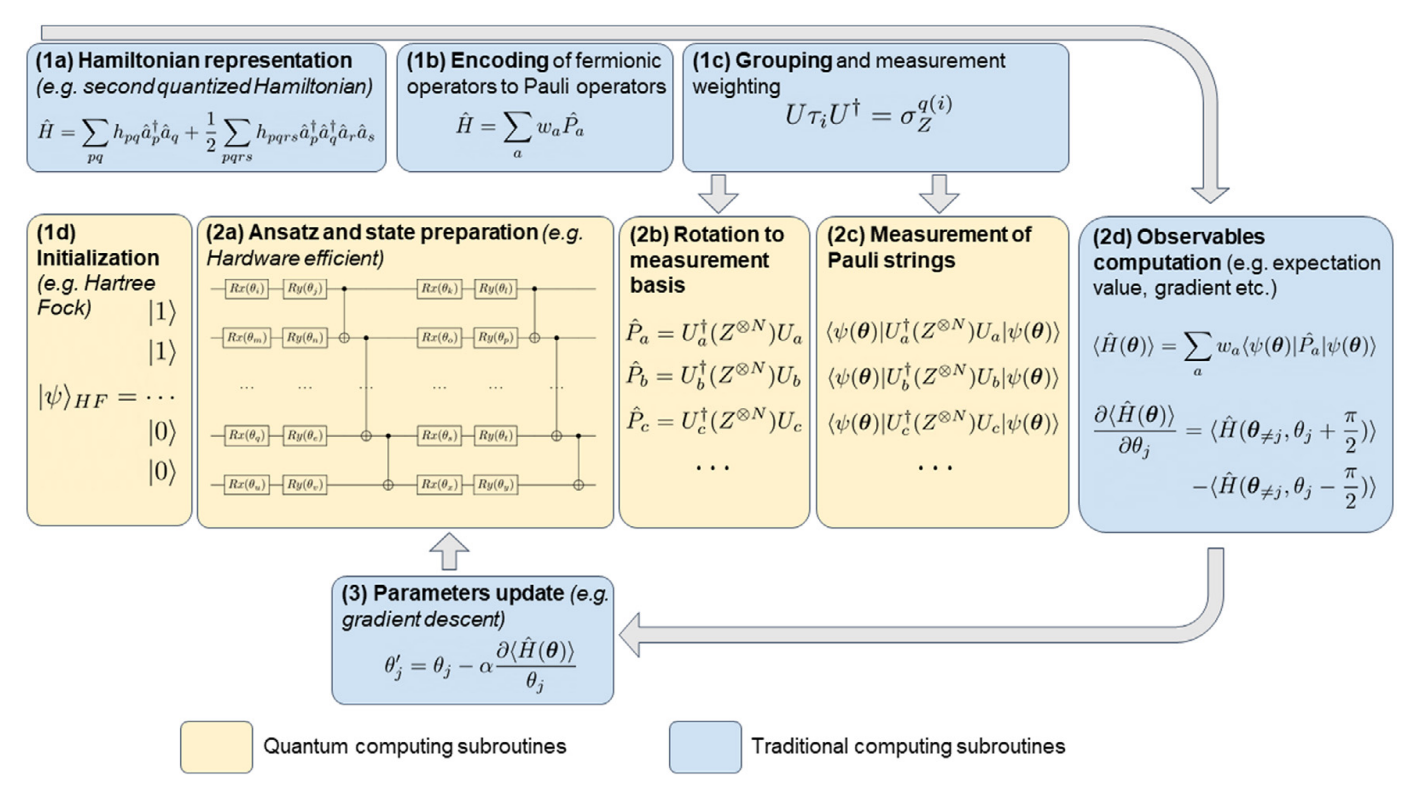
\includegraphics[width=\textwidth]{Images/VQE_diagram.png}
        \caption{Shrnutí VQE, ukradeno z \cite{tilly_variational_2022}, ideálně PŘEKRESLIT do vektoru a udělat hezčí.}
        \label{fig:VQE_diagram}
    \end{figure}
\section{Popis algoritmu}
Jak již bylo 
\section{Ansatz}
\section{Enkódování Hamiltoniánu}
\subsection{Druhé kvantování}
Popisuje přepis Hamiltoniánu do tzv. notace obsazovacích čísel

Mějme $N$ částic. $n_i$ odpovídá počtu částic ve stavu $i$. Libovolný stav $\mathcal{F}^N$ lze zapsat následující superpozicí
\begin{equation}
    \ket{\psi} = \sum_{\sum n_i = N} C_{n_1, n_2,..}\ket{n_1, n_2,...}
\end{equation}
Prostor $\mathcal{F} = \otimes_{N=0}^{\infty} F^N$ je Fockův prostor...libovolný počet částic. $\{ \ket{n_1, n_2,...} \}$ je báze. Libovolný vektor:
\begin{equation}
    \ket{\psi} = \sum_{n_1,n_2,..} C_{n_1, n_2,..}\ket{n_1, n_2,...}
\end{equation}
Definujeme posunovací operátory
\begin{equation}
    a^\dag_i \ket{n_1,...,n_i,...} = \sqrt{n_i+1} \xi^{s_i} \ket{n_1,...,n_i+1,...}
\end{equation}
Bázi lze vygenerovat
\begin{equation}
    \ket{n_1,n_2,..} = \prod_i \tfrac{1}{\sqrt{n_i!}} (a^\dag_i)^{n_i} \ket{0}
\end{equation}

Lze odvodit, že
\begin{equation}
    a^\dag_i \ket{n_1,...,n_i,...} = \sqrt{n_i} \xi^{s_i} \ket{n_1,...,n_i-1,...}
\end{equation}

Přejdeme k od čísel k $\lambda$. Operátor $\hat{a}^\dag_\lambda$ vytvoří částici ve stavu $\lambda$

\subsubsection{Reprezentace jednočásticových operátorů}
Jednočásticový operátor často ve tvaru:
\begin{equation}
    \hat{O} = \sum_{n=1}^N \hat{o}_n,
\end{equation}
je jím např. nerelativistická kinetická energie $\hat{T} = \sum \tfrac{\hat{p}^2}{2m}$
Zavádíme operátor počtu částic
\begin{equation}
    \hat{n}_\lambda = \hat{a}^\dag_\lambda\hat{a}_\lambda
\end{equation}

\subsection{Jordan-Wiegnerova transformace}
\section{Měření}
\subsection{Pauliho řetězce}
\subsection{Diagonalizace}
\subsection{Seskupení}
\label{sec:pauli_grouping}
\section{Optimizéry}
\subsection{Gradientní}
\subsection{Negradientní}
\section{Modifikace a budoucnost}
\subsection{Excitované stavy}
\subsection{Folded Spectrum VQE}
\subsection{Cascaded VQE}





\chapter{Kvarkonia (Vektorové mezony)}

\pagestyle{headings}


\part{Praktická část}



\chapter*{Závěr}
\addcontentsline{toc}{chapter}{Závěr}

\pagestyle{plain}

To be continued....

\printbibliography
\addcontentsline{toc}{chapter}{Bibliografie}

\end{document}
